%%%%%%%%%%%%%%%%%%%%%%%%%%%%%%%%%%%%%%%%%%%%%%%%%%%%%%%%%%%%%%%%
%%%%%%%%%%%%%%%%%%%%%%%%%%%%%%%%%%%%%%%%%%%%%%%%%%%%%%%%%%%%%%%%
%%%%
%%%% This text file is part of the source of slides for
%%%% `Introduction to High-Performance Scientific Computing'
%%%% by Victor Eijkhout, copyright 2012
%%%%
%%%%%%%%%%%%%%%%%%%%%%%%%%%%%%%%%%%%%%%%%%%%%%%%%%%%%%%%%%%%%%%%
%%%%%%%%%%%%%%%%%%%%%%%%%%%%%%%%%%%%%%%%%%%%%%%%%%%%%%%%%%%%%%%%

\documentclass[headnav]{beamer}

\newenvironment{beamdisplayeq}%
 {\begin{equation}\small}{\end{equation}}

\usepackage{beamerthemeTACC}
\parskip=.5\baselineskip plus .5\baselineskip
\event{Intro sci/tech computing}

\usepackage{graphicx,comment,multicol,undertilde}
\usepackage{hyperref}

\newcommand\inv{^{-1}}

\begin{document}
\title{Ordinary and partial differential equations}
\author{Victor Eijkhout}
\date{335/394 fall 2011}
\frame{\titlepage}

\frame{\frametitle{ODEs and PDEs}
Time-evolving phenomena:
IVP (Initial Value Problem), usually Ordinary Differential Equations

Space-constraint phenomena:
BVP (Boundary Value Problem), usually Partial Differential Equations

}

\sectionframe{Ordinary Differential Equations}

\frame{\frametitle{Numerical treatment of differential equations}

  Initial value problem: $u'(t)=f(t,u(t)),\qquad u(0)=u_0,\qquad t>0$

  Boundary value problem: $u''(x)=f(x),\qquad x(0)=x_0,x(1)=x_1,\qquad x\in[0,1] $

  General assumption: $f$ has higher derivatives.

  IVP stability: solutions corresponding to different $u_0$ values converge
  as $t\rightarrow\infty$. Criterium:
  \[ \frac\partial{\partial u}f(t,u)=
  \begin{cases}
    >0&unstable\\ =0&neutrally stable\\ <0&stable
  \end{cases}
  \]
  Simple example: $f(t,u)=-\lambda u$, then $u(t)=u_0e^{-\lambda t}$;\\
  stable if $\lambda>0$
}

\frame{\frametitle{proof}

Let $u^*$ s.t. $f(u^*)=0$, then $u(t)\equiv u^*$ is a solution of $u'=f(u)$,

Write solutions as $u(t)=u^*+\eta(t)$, then 
\[
\begin{array}{rl}
  \eta'&=u'=f(u)=f(u^*+\eta)=f(u^*)+\eta f'(u^*)+O(\eta^2)\\
     &=\eta f'(u^*)+O(\eta^2)
\end{array}
\]
Ignoring the second order terms, this has the solution
\[ \eta(t)=e^{f'(u^*)t} \]
which means that the perturbation will damp out if $f'(u^*)<0$.

}
\frame{\frametitle{Finite difference approximation}

  We turn the continuous problem into a discrete one, by looking at finite
  time/space steps.

  Assume all functions are sufficiently smooth, and use Taylor series:
  \[ u(t+\Delta t)=u(t)+u'(t)\Delta t+u''(t)\frac{\Delta t^2}{2!}
  + u'''(t)\frac{\Delta t^3}{3!}+\cdots \]
  This gives for $u'$:
  \[ u'(t) = \frac{u(t+\Delta t)-u(t)}{\Delta t}+O(\Delta t^2) \]
  So we approximate
  \[ u'(t)\approx \frac{u(t+\Delta t)-u(t)}{\Delta t} \]
  and the ``truncation error'' is $O(\Delta t^2)$.
}

\frame{\frametitle{Finite differences 2}

  How does this help? In $u'=f(t,u)$ substitute
  \[ u'(t)\rightarrow \frac{u(t+\Delta t)-u(t)}{\Delta t} \]
  giving
  \[ \frac{u(t+\Delta t)-u(t)}{\Delta t} = f(t,u(t)) \]
  or 
  \[ u(t+\Delta t) = u(t) + \Delta t\,f(t,u(t)) \]
  Let $t_0=0$, $t_{k+1}=t_k+\Delta t=\cdots=(k+1)\Delta t$, $u(t_k)=u_k$:
  \[ u_{k+1}=u_k+\Delta t\,f(t_k,u_k) \]
  Discretization\\`Explicit Euler' or `Euler forward'.

  Does this compute something close to the true solution?\\
  `Discretization error'
}

\frame{\frametitle{Some error analysis}

  Local Truncation Error: assume computed solution is exact at step~$k$, 
  how wrong will we be at step~$k+1$?
  \begin{eqnarray*}
    u(t_{k+1})&=&u(t_k)+u'(t_k)\Delta t+u''(t_k)\frac{\Delta t^2}{2!}+\cdots\\
    &=&u(t_k)+f(t_k,u(t_k))\Delta t+u''(t_k)\frac{\Delta t^2}{2!}+\cdots\\
    u_{k+1}&=&u_k+f(t_k,u_k)\Delta t    
  \end{eqnarray*}
  So 
  \begin{eqnarray*}    
  L_{k+1}&=&u_{k+1}-u(t_{k+1})\\
  &=&u_k-u(t_k)+f(t_k,u_k)-f(t_k,u(t_k))
  -u''(t_k)\frac{\Delta t^2}{2!}+\cdots\\
  &=&-u''(t_k)\frac{\Delta t^2}{2!}+\cdots
  \end{eqnarray*}
  Global error: $E_k\approx\Sigma_k L_k=k\Delta t\frac{\Delta t^2}{2!}
  =O(\Delta t)$:
  First order method
}

\frame{\frametitle{An Euler forward example}

  Consider $f(t,u)=-\lambda u$, exact solution $u(t)=u_0e^{-\lambda t}$;\\
  stable if $\lambda>0$

  Explicit Euler scheme
  \[ u_{k+1}=u_k-\Delta t \lambda u_k=(1-\lambda \Delta t)u_k
  =(1-\lambda\Delta t)^ku_0 \]
  Then
  \begin{eqnarray*}
    &&\hbox{$u_k\rightarrow 0$ as $k\rightarrow\infty$}\\
    &\Leftrightarrow&|1-\lambda \Delta t|<1\\
    &\Leftrightarrow&-1<1-\lambda\Delta t<1\\
    &\Leftrightarrow&-2<-\lambda\Delta t<0\\
    &\Leftrightarrow&0<\lambda\Delta t<2\\
    &\Leftrightarrow&\Delta t<2/\lambda
  \end{eqnarray*}
  Conditionally stable
}

\frame{\frametitle{Implicit Euler}

  Or `Euler backward':
  \[ u(t-\Delta t)=u(t)-u'(t)\Delta t+u''(t)\frac{\Delta t^2}{2!}+\cdots \]
  so
  \[ u'(t)=\frac{u(t)-u(t-\Delta t)}{\Delta t}+u''(t)\Delta t/2+\cdots \]
  Compute $u'(t)=f(t,u(t))$ as
  \begin{eqnarray*}
    &&\frac{u(t)-u(t-\Delta t)}{\Delta t}=f(t,u(t))\\
    &\Rightarrow&u(t)=u(t-\Delta t)+\Delta t f(t,u(t))\\
    &\Rightarrow&u_{k+1}=u_k+\Delta tf(t_{k+1},u_{k+1})
  \end{eqnarray*}
  Implicit equation for $u_{k+1}$!

  Let $f(t,u)=-u^3$, then $u_{k+1}=u_k-\Delta t u_{k+1}^3$\\
  needs nonlinear solver
}

\frame{\frametitle{Stability of Implicit Euler}

  Again the $f(t,u)=-\lambda u$ example:
  \[
  \begin{array}{l}
    u_{k+1} = u_k-\lambda \Delta t u_{k+1}\\
    (1+\lambda\Delta t)u_{k+1}=u_k\\
    u_{k+1}=\left (\frac1{1+\lambda\Delta t}\right)u_k
    =\left (\frac1{1+\lambda\Delta t}\right)^ku_0
  \end{array}
  \]
  If $\lambda>0$ (stable equation), then $u_k\rightarrow0$ for all values
  of $\lambda$ and~$\Delta t$: unconditionally stable.

  Pro: larger time steps possible, no worries\\
  Con: implicit equation needs to be solved
}

\frame{\frametitle{Higher order methods}

  Runge-Kutta\\
  Adams-Bashforth\\
  Crank-Nicholson
}

\frame{\frametitle{Boundary value problems}
  Consider $u''(x)=f(x,u,u')$ for $x\in[a,b]$ where $u(a)=u_a$, $u(b)=u_b$
in 1D and
\begin{equation}
 \hbox{$-u_{xx}(\bar x)-u_{yy}(\bar x)=f(\bar x)$ for
   $x\in\Omega=[0,1]^2$ 
    with $u(\bar x)=u_0$ on $\delta\Omega$.}
 \label{eq:2nd-order-bvp-2D}
 \end{equation}
in 2D.
}
\frame{\frametitle{Approximation of 2nd order derivatives}
\footnotesize
  Taylor series (write $h$ for $\delta x$):
  \[ u(x+h)=u(x)+u'(x)h+u''(x)\frac{h^2}{2!}+u'''(x)\frac{h^3}{3!}
  +u^{(4)}(x)\frac{h^4}{4!}+u^{(5)}(x)\frac{h^5}{5!}+\cdots \]
  and
  \[ u(x-h)=u(x)-u'(x)h+u''(x)\frac{h^2}{2!}-u'''(x)\frac{h^3}{3!}
  +u^{(4)}(x)\frac{h^4}{4!}-u^{(5)}(x)\frac{h^5}{5!}+\cdots \]
  Subtract:
  \[ u(x+h)+u(x-h)=2u(x)+u''(x)h^2+u^{(4)}(x)\frac{h^4}{12}+\cdots \]
  so
  \[ u''(x)=\frac{u(x+h)-2u(x)+u(x-h)}{h^2}-u^{(4)}(x)\frac{h^4}{12}+\cdots \]


  Numerical scheme:
  \[ -\frac{u(x+h)-2u(x)+u(x-h)}{h^2}=f(x,u(x),u'(x)) \]
  (2nd order PDEs are very common!)
}

\frame{\frametitle{This leads to linear algebra}
  \[ -\frac{u(x+h)-2u(x)+u(x-h)}{h^2}=f(x,u(x),u'(x)) \]
  Equally spaced points on $[0,1]$: $x_k=kh$ where $h=1/n$, then
  \[ -u_{k+1}+2u_k-u_{k-1} = h^2\,f(x_k,u_k,u'_k)
  \quad\hbox{for $k=1,\ldots,n-1$} \]
  Written as matrix equation:
  \[
  \left(
    \begin{matrix}
      2&-1\\ -1&2&-1\\ &\ddots&\ddots&\ddots
    \end{matrix}\right)
  \left(
    \begin{matrix}
      u_1\\ u_2\\ \vdots
    \end{matrix}\right)
  = 
  \left(
    \begin{matrix}
      h^2f_1+u_0\\ h^2f_2\\ \vdots
    \end{matrix}\right)
  \]
}

\frame{\frametitle{Matrix properties}

  \begin{itemize}
  \item Very sparse, banded
  \item Symmetric (only because 2nd order problem)
  \item Sign pattern: positive diagonal, nonpositive off-diagonal\\
    (true for many second order methods)
  \item Positive definite (just like the continuous problem)
  \end{itemize}
}

\frame{\frametitle{Initial Boundary value problem}
  Heat conduction in a rod $T(x,t)$ for $x\in[a,b]$, $t>0$:
  \[ \frac\partial{\partial t}T(x,t)-\alpha\frac{\partial^2}{\partial x^2}T(x,t)
  =q(x,t) \]
  \begin{itemize}
  \item Initial condition: $T(x,0)=T_0(x)$
  \item Boundary conditions: $T(a,t)=T_a(t)$, $T(b,t)=T_b(t)$
  \item Material property: $\alpha>0$ is thermal diffusivity
  \item Forcing function: $q(x,t)$ is externally applied heating.
  \end{itemize}
  The equation $u''(x)=f$ above is the steady state.
}

\frame{\frametitle{Discretization}
  Space discretization: $x_0=a$, $x_n=b$, $x_{j+1}=x_j+\Delta x$\\
  Time discretiation: $t_0=0$, $t_{k+1}=t_k+\Delta t$\\
  Let $T^k_j$ approximate $T(x_j,t_k)$

  Space:
  \[ \frac\partial{\partial t}T(x_j,t)-\alpha
  \frac{T(x_{j-1},t)-2T(x_j,t)+T(x_{j+1},t)}{\Delta x^2}=q(x_j,t) \]
  Explicit time stepping:
  \[ \frac{T_j^{k+1}-T_j^k}{\Delta t}-\alpha
  \frac{T_{j-1}^k-2T_j^k+T_{j+1}^k}{\Delta x^2}=q_j^k \]
  Implicit time stepping:
  \[ \frac{T_j^{k+1}-T_j^k}{\Delta t}-\alpha
  \frac{T_{j-1}^{k+1}-2T_j^{k+1}+T_{j+1}^{k+1}}{\Delta x^2}=q_j^{k+1} \]
}

\frame{\frametitle{Computational form:   explicit}
  \[ T_j^{k+1}=T_j^k+\frac{\alpha\Delta t}{\Delta x^2}
  (T_{j-1}^k-2T_j^k+T_{j+1}^k)+\Delta t q_j^k \]
  This has an explicit form:
  \[ \utilde T^{k+1}=\left(I+\frac{\alpha\Delta t}{\Delta x^2}\right
  )\utilde T^k+\Delta t\utilde q^k \]
}

\frame{\frametitle{Computational form: implicit}
  \[ T_j^{k+1}-\frac{\alpha\Delta t}{\Delta x^2}
  (T_{j-1}^k-2T_j^k+T_{j+1}^k)=T_j^k+\Delta t q_j^k \]
  This has an implicit form:
  \[ \left(I-\frac{\alpha\Delta t}{\Delta x^2}K\right)\utilde T^{k+1}=
  \utilde T^k+\Delta t\utilde q^k \]
  Needs to solve a linear system in every time step
}
\def\fr{\frac{\alpha\Delta t}{\Delta x^2}}
\frame{\frametitle{Stability of explicit scheme}
  Let $q\equiv0$; assume $T_j^k=\beta^ke^{i\ell x_j}$; for stability
  we require $|\beta|<1$:
  \begin{eqnarray*}
    T_j^{k+1}&=&T_j^k+\fr(T_{j-1}^k-2T_j^k+T_{j+1}^k)\\
    \Rightarrow \beta^{k+1}e^{i\ell x_j}&=&\beta^ke^{i\ell x_j}
    +\fr (\beta^ke^{i\ell x_{j-1}}-2\beta^ke^{i\ell x_j}+\beta^ke^{i\ell x_{j+1}})\\
    \Rightarrow \beta&=&
    1+2\fr[\frac12(e^{i\ell\Delta x}+e^{-\ell\Delta x})-1]\\
    &=&1+2\fr(\cos(\ell\Delta x)-1)
  \end{eqnarray*}
}

\frame{
  \[  \frac{\beta^{k+1}}{\beta^k}=
  1+2\fr(\cos(\ell\Delta x)-1) \]
  To get $|\beta|<1$:
  \begin{itemize}
  \item $2\fr(\cos(\ell\Delta x)-1)<0$: automatic
  \item $2\fr(\cos(\ell\Delta x)-1)>-2$: needs $2\fr<1$, that is
    \[ \Delta t<\frac{\Delta x^2}{2\alpha} \]
    big restriction on size of time steps
  \end{itemize}
}

\frame{\frametitle{Stability of implicit scheme}
  \small
  \begin{eqnarray*}
    T_j^{k+1}-\fr(T_{j_1}^{k+1}-2T_j^{k+1}+T_{j+1}^{k+1})&=&T_j^k\\
    \Rightarrow \beta^{k+1}e^{i\ell \Delta x}-\fr
    (\beta^{k+1}e^{i\ell x_{j-1}}-2\beta^{k+1}e^{i\ell x_j}
    +\beta^{k+1}e^{i\ell x_{j+1}})&=&\beta^ke^{i\ell x_j}
  \end{eqnarray*}
  \begin{eqnarray*}
    \Rightarrow \beta\inv&=&1+2\fr(1-\cos(\ell\Delta x))\\
    \beta&=&\frac1{1+2\fr(1-\cos(\ell\Delta x))}
  \end{eqnarray*}
  Noting that $1-\cos(\ell\Delta x)>0$, 
  the condition $|\beta|<1$ always satisfied:
  method always stable.
}

\frame{\frametitle{Sparse matrix in 2D case}
Sparse matrices so far were tridiagonal: only in 1D case.

Two-dimensional: $-u_{xx}-u_{yy}=f$ on unit square $[0,1]^2$

Difference equation: {\small $4u(x,y)-u(x+h,y)-u(x-h,y)-u(x,y+h)-u(x,y-h)=h^2f(x,y)$}

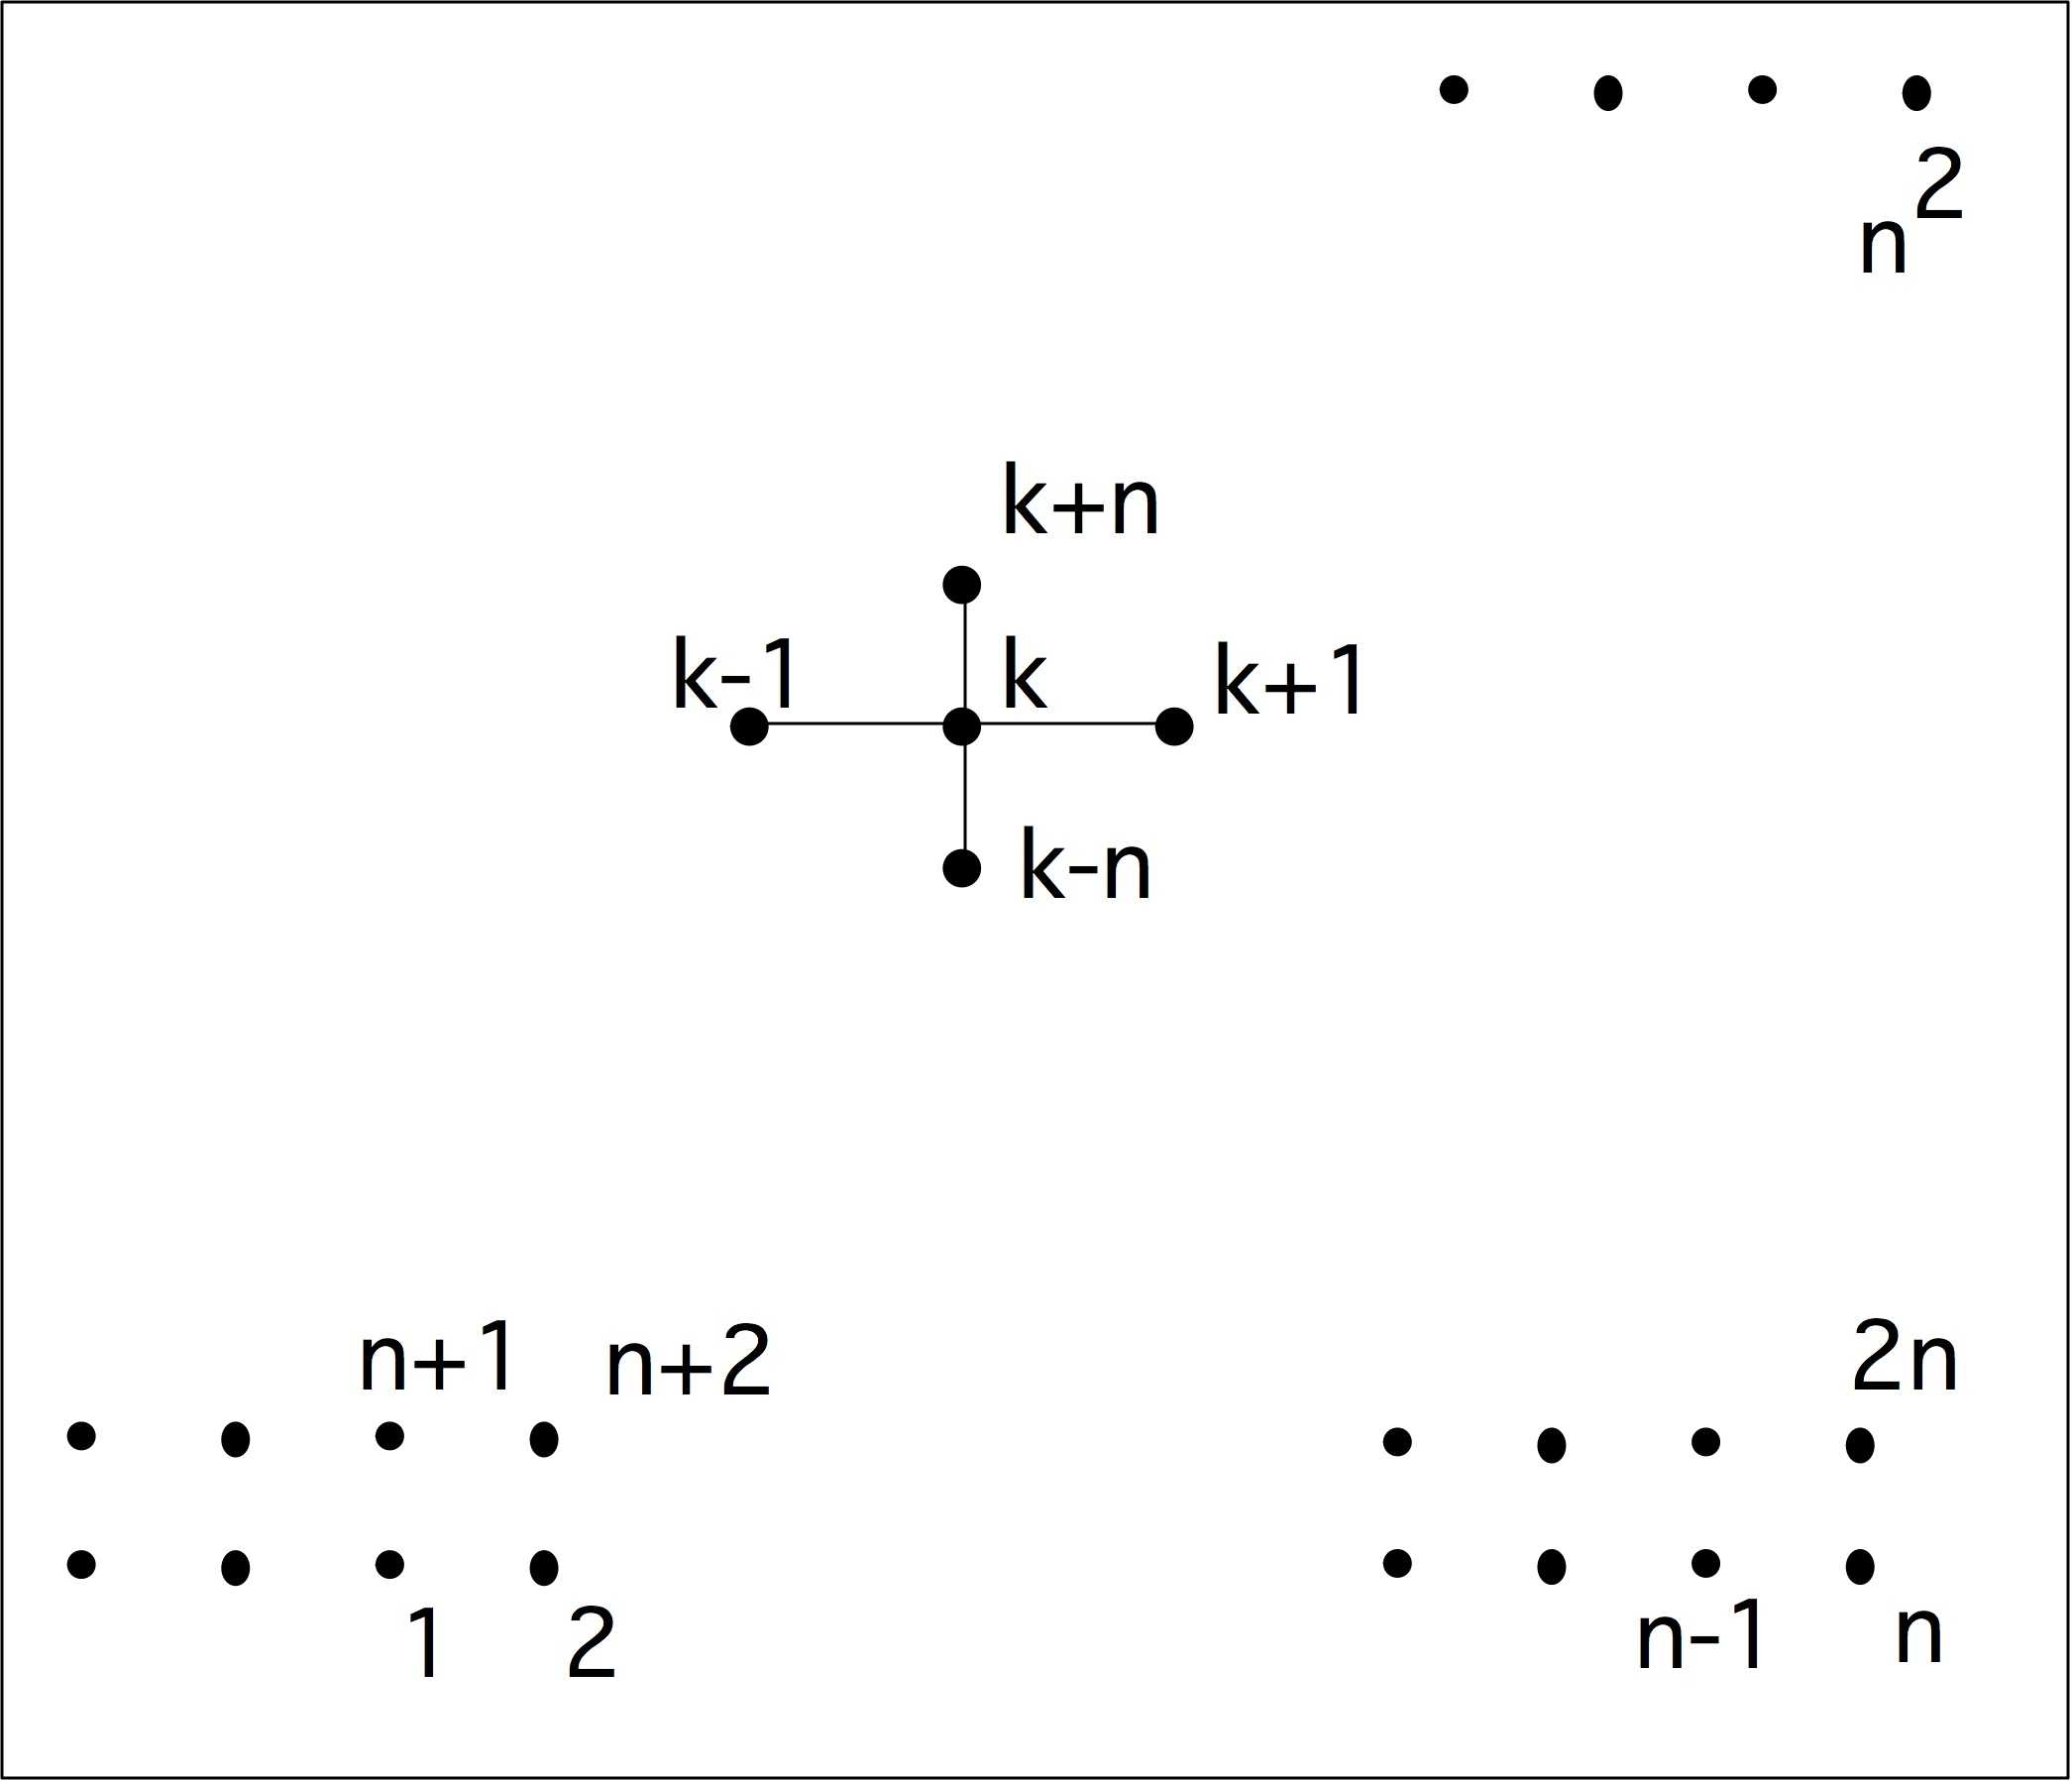
\includegraphics[scale=.07]{graphics/laplacedomain}
}

\frame{\frametitle{Sparse matrix from 2D equation}
\small
\[
  \left(\begin{array}{ccccc|ccccc|cc}
    4&-1&&&\emptyset&-1&&&&\emptyset&\\ 
    -1&4&1&&&&-1&&&&\\ 
    &\ddots&\ddots&\ddots&&&&\ddots&&\\ 
    &&\ddots&\ddots&-1&&&&\ddots&\\ 
    \emptyset&&&-1&4&\emptyset&&&&-1&\\ \hline
    -1&&&&\emptyset&4&-1&&&&-1\\
    &-1      &      &&&-1      &4       &-1      &&&&-1\\
    &\uparrow&\ddots&&&\uparrow&\uparrow&\uparrow&&  &&\uparrow\\
    &k-n     &      &&&k-1     &k       &k+1     &&-1&&k+n\\
    &&&&-1&&&&-1&4&&\\ \hline
    &        &      &&&\ddots  &        &        &&  &\ddots\\
  \end{array}\right)
\]
}

\end{document}
